\documentclass[a4paper,twoside]{article}
\usepackage[T1]{fontenc}
\usepackage[bahasa]{babel}
\usepackage{graphicx}
\usepackage{graphics}
\usepackage{float}
\usepackage[cm]{fullpage}
\pagestyle{myheadings}
\usepackage{etoolbox}
\usepackage{setspace} 
\usepackage{lipsum} 
\setlength{\headsep}{30pt}
\usepackage[inner=2cm,outer=2.5cm,top=2.5cm,bottom=2cm]{geometry} %margin
% \pagestyle{empty}

\makeatletter
\renewcommand{\@maketitle} {\begin{center} {\LARGE \textbf{ \textsc{\@title}} \par} \bigskip {\large \textbf{\textsc{\@author}} }\end{center} }
\renewcommand{\thispagestyle}[1]{}
\markright{\textbf{\textsc{Laporan Perkembangan Pengerjaan Skripsi\textemdash Sem. Ganjil 2015/2016}}}

\onehalfspacing
 
\begin{document}

\title{\@judultopik}
\author{\nama \textendash \@npm} 

%ISILAH DATA DATA BERIKUT INI:
\newcommand{\nama}{Billy Yanuar}
\newcommand{\@npm}{2012730017}
\newcommand{\tanggal}{21/11/2016} %Tanggal pembuatan dokumen
\newcommand{\@judultopik}{Sistem Penilaian Sidang Skripsi 2 Dengan AngularJS} % Judul/topik anda
\newcommand{\kodetopik}{PAS4004}
\newcommand{\jumpemb}{1} % Jumlah pembimbing, 1 atau 2
\newcommand{\pembA}{Pascal Alfadian}
\newcommand{\pembB}{-}
\newcommand{\semesterPertama}{41 - Ganjil 16/17} % semester pertama kali topik diambil, angka 1 dimulai dari sem Ganjil 96/97
\newcommand{\lamaSkripsi}{1} % Jumlah semester untuk mengerjakan skripsi s.d. dokumen ini dibuat
\newcommand{\kulPertama}{Skripsi 1} % Kuliah dimana topik ini diambil pertama kali
\newcommand{\tipePR}{C} % tipe progress report :
% A : dokumen pendukung untuk pengambilan ke-2 di Skripsi 1
% B : dokumen untuk reviewer pada presentasi dan review Skripsi 1
% C : dokumen pendukung untuk pengambilan ke-2 di Skripsi 2
\maketitle

\pagenumbering{arabic}

\section{Data Skripsi} %TIDAK PERLU MENGUBAH BAGIAN INI !!!
Pembimbing utama/tunggal: {\bf \pembA}\\
Pembimbing pendamping: {\bf \pembB}\\
Kode Topik : {\bf \kodetopik}\\
Topik ini sudah dikerjakan selama : {\bf \lamaSkripsi} semester\\
Pengambilan pertama kali topik ini pada : Semester {\bf \semesterPertama} \\
Pengambilan pertama kali topik ini di kuliah : {\bf \kulPertama} \\
Tipe Laporan : {\bf \tipePR} -
\ifdefstring{\tipePR}{A}{
			Dokumen pendukung untuk {\BF pengambilan ke-2 di Skripsi 1} }
		{
		\ifdefstring{\tipePR}{B} {
				Dokumen untuk reviewer pada presentasi dan {\bf review Skripsi 1}}
			{	Dokumen pendukung untuk {\bf pengambilan ke-2 di Skripsi 2}}
		}

\section{Detail Perkembangan Pengerjaan Skripsi}
Detail bagian pekerjaan skripsi sesuai dengan rencana kerja/laporan perkembangan terkahir :
	\begin{enumerate}
		\item Mempelajari komponen-komponen dan variabel - variabel yang perlu disimpan pada lembar penilaian skripsi yang dipakai saat ini \\
		{\bf status :} Ada sejak rencana kerja skripsi.\\
		{\bf hasil :} Untuk mengetahui isi dan variabel - variabel yang dibutuhkan untuk penyimpanan sistem penilaian sidang skripsi 2 ini, diperlukan contoh lembaran form penilaian sidang skripsi 2 yang sekarang dipakai pada Program Studi Teknik Informatika di Universitas Katolik Parahyangan. Form penilaian tersebut sudah berhasil didapatkan berdasarkan izin dari dosen pembimbing dan juga ketua jurusan Program Studi Teknik Informatika di Universitas Katolik Parahyangan. Berdasarkan form tersebut dan diskusi dengan dosen pembimbing, maka dapat disimpulkan bahwa sistem penilaian sidang skripsi 2 pada Program Studi Teknik Informatika di Universitas Katolik Parahyangan hanya membutuhkan satu buah tabel dengan 29 variabel yang perlu disimpan.\\
		Variabel - variabel tersebut meliputi: tahun, semester, npm, nama, judul skripsi, nama pembimbing, nama ketua tim penguji, nama anggota tim penguji, bobot ketua tim penguji, bobot anggota tim penguji, bobot pembimbing, nilai koodinator skripsi, bobot koordinator skripsi, bobot tata tulis laporan anggota tim penguji, bobot kelengkapan materi anggota tim penguji, bobot penguasaan materi anggota tim penguji, bobot presentasi anggota tim penguji, bobot pencapaian tujuan anggota tim penguji, bobot tata tulis laporan ketua tim penguji, bobot kelengkapan materi ketua tim penguji, bobot penguasaan materi ketua tim penguji, bobot presentasi ketua tim penguji, bobot pencapaian tujuan ketua tim penguji, bobot tata tulis laporan pembimbing, bobot kelengkapan materi pembimbing, bobot penguasaan materi pembimbing, bobot proses bimbingan pembimbing, dan nilai akhir mahasiswa. Nilai - nilai selain ke 29 hal itu tidak diperlukan untuk disimpan karena bisa dihitung dari data nilai akhir dan bobot yang tersimpan pada basis data.\\
		Gambar \ref{fig:database} adalah tabel basis data dari komponen-komponen dan variabel-variabel yang perlu disimpan di basis data dengan "id" sebagai \textit{primary key} yang diberikan fungsi "\textit{auto\_increment}" yaitu secara otomatis mengisi baru jika ada data yang ditambahkan.
		
			\begin{figure}[H]
				\centering
				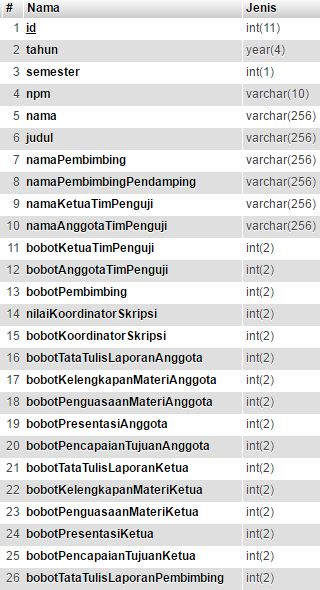
\includegraphics[scale=0.75]{Gambar/database1}
				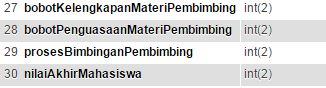
\includegraphics[scale=0.75]{Gambar/database2}
				\caption{Variabel yang disimpan di database}
				\label{fig:database}
			\end{figure}
		
		\item Mempelajari bahasa pemrograman AngularJS, Code Igniter, dan Bootstrap\\
		{\bf status :} Ada sejak rencana kerja skripsi.\\
		{\bf hasil :} Dalam proses pembelajaran, \textit{framework} pertama yang saya pelajari adalah CodeIgniter, karena \textit{framework} ini merupakan framework PHP dengan Model, View, dan Controller (MVC) yang menjadi dasar dari struktur dan pemanggilan file - file dengan menggunakan PHP pada sistem penilaian sidang skripsi 2 ini. Tujuan penggunaan CodeIgniter sendiri adalah untuk mempermudah dan mempercepat \textit{developer} dalam pengembangan aplikasi, dibandingkan dengan membuatnya dari awal. CodeIgniter menyediakan banyak \textit{library} yang berupa kumpulan \textit{task} umum yang biasa dipakai, \textit{interface} sederhana, dan juga stuktur - struktur logika yang sudah disiapkan untuk pengaksesan \textit{library}.
		\linebreak
		Selanjutnya saya mempelajari Bootstrap. Bootstrap merupakan sebuah alat bantu untuk membuat sebuah tampilan halaman website yang dapat mempercepat pekerjaan seorang pengembang website ataupun pendesain halaman website. Dasar dari Bootstrap sendiri adalah kumpulan class CSS dan \textit{plugin} JavaScript yang sudah siap untuk dipakai pada sebuah halaman HTML. Karena sebelumnya saya sempat memakai \textit{foundation zurb}, maka saya tidak terlalu mengalami kesulitan dalam proses pembelajaran bootstrap karena kemiripan cara kerja dari kedua \textit{framework} tersebut.\\
		\linebreak
		Setelah selesai menguasai kedua framework tersebut barulah saya mempelajari AngularJS. AngularJS merupakan sebuah \textit{web-application-framework} yang berfokus pada \textit{web-based single-page application} dimana fitur-fitur yang ada pada aplikasi web dapat berjalan dengan menggunakan sebuah halaman HTML tanpa perlu berganti halaman. AngularJS bekerja dengan membaca HTML page yang sudah diberi \textit{tag} tambahan khusus yang berfungsi untuk mulai mengeksekusi AngularJS, seperti ng-app, ng-model, ng-controller, dll. AngularJS memanfaatkan \textit{tag} tersebut sebagai atribut input dan output yang direpresentasikan oleh javascript biasa. 
		Dari pembelajaran tersebutlah Sistem Penilaian Sidang Skripsi 2 dengan AngularJS berhasil dibuat.\\
		Saat ini, pembuatan aplikasi sistem penilaian sidang skripsi 2 sudah berhasil dibuat dengan menggunakan ketika \textit{framework} yang sudah dipelajari di atas. Seluruh fitur pun sudah berjalan dengan baik dan penyimpanan pada database menggunakan CodeIgniter sudah dapat berjalan dengan baik tanpa adanya kesalahan atau \textit{error} yang terjadi pada aplikasi. Aplikasi pun sudah menggunakan \textit{web-hosting} dari Qwords. Aplikasi sistem penilaian sidang skripsi 2 dengan AngularJS dapat dijalankan secara online dengan URL "sipskripsi.com".

		\item Merancang tampilan form yang akan dipakai untuk penilaian\\
		{\bf status :} Ada sejak rencana kerja skripsi.\\
		{\bf hasil :} Tampilan form mulai dirancang ketika saya selesai belajar CodeIgniter dan Bootstrap. Tampilan form sistem penilaian sidang skripsi 2 ini merupakan pengembangan dari \textit{template} dasar bootstrap bernama scrolling-nav dengan versi 1.04 yang saya dapatkan dengan mengunduh file zip dari "http://startbootstrap.com/template-categories/all/" . Saya memilih template ini dengan mempertimbangkan beberapa alasan yang sangat vital untuk form sistem penilaian sidang skripsi 2, diantaranya adalah sistem yang dibuat memakai AngularJS memiliki keunggulan pada \textit{single-page application}, diperlukan sebuah form yang menggabungkan seluruh lembar form penilaian dan lembar form rekapitulasi, dibutuhkannya navigasi sebagai bantuan untuk user dalam meletakkan nilai-nilai yang diperlukan. Oleh karena itu, template \textit{scrolling-nav} ini merupakan sebuah template yang sangat cocok dan memenuhi syarat untuk sistem penilaian sidang skripsi 2 ini. Ditambah lagi dengan navigasi yang menunjukkan tempat yang diinginkan dengan efek seperti penggunaan \textit{scroll} pada mouse akan menambah nilai keunikan tersendiri pada sistem penilaian sidang skripsi 2 ini.\\
		Gambar\ref{fig:tampilan} merupakan rancangan tampilan yang sudah dibuat.\\
		
			\begin{figure}[H]
				\centering
				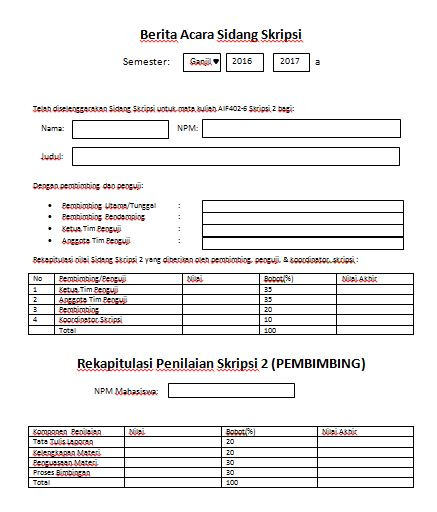
\includegraphics[scale=0.75]{Gambar/tampilan1}
				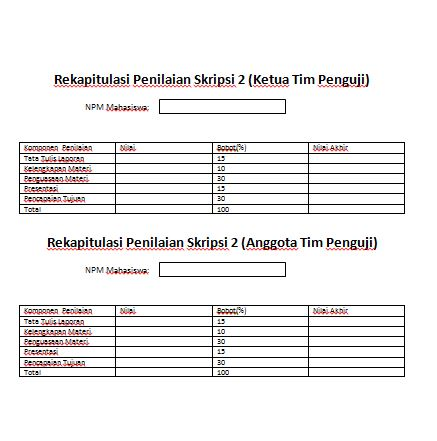
\includegraphics[scale=0.75]{Gambar/tampilan2}
				\caption{Gambar Rancangan Tampilan Aplikasi}
				\label{fig:tampilan}
			\end{figure}
		
		Dari rancangan tersebut, jadilah tampilan program pada gambar \ref{fig:tampilanapp}.\\
		
			\begin{figure}[H]
				\centering
				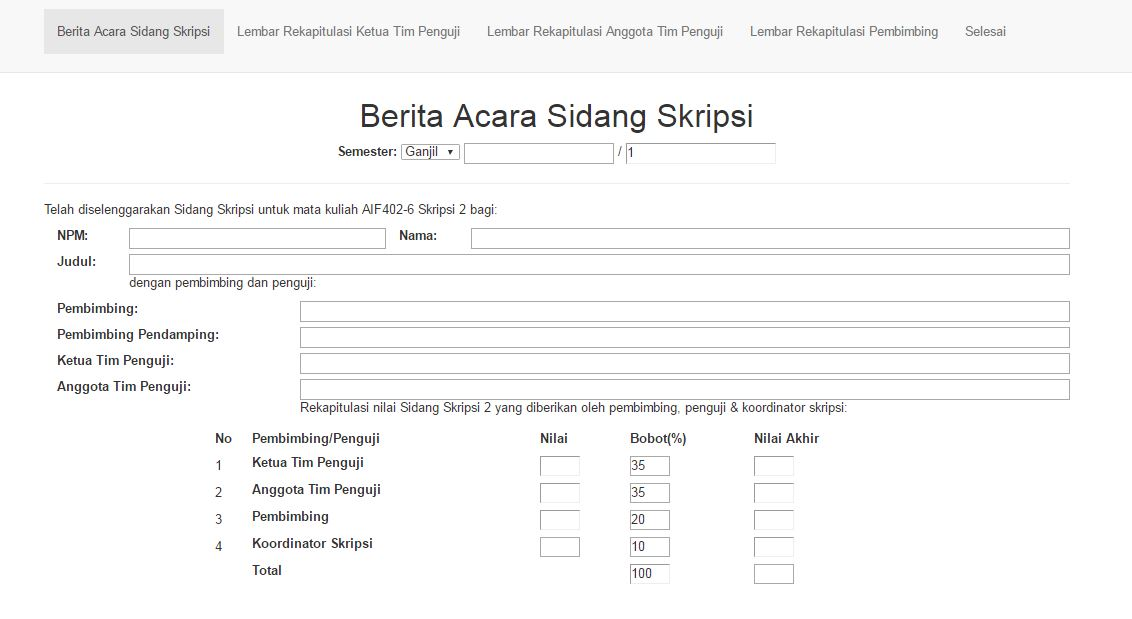
\includegraphics[scale=0.5]{Gambar/tampilanapp1}
				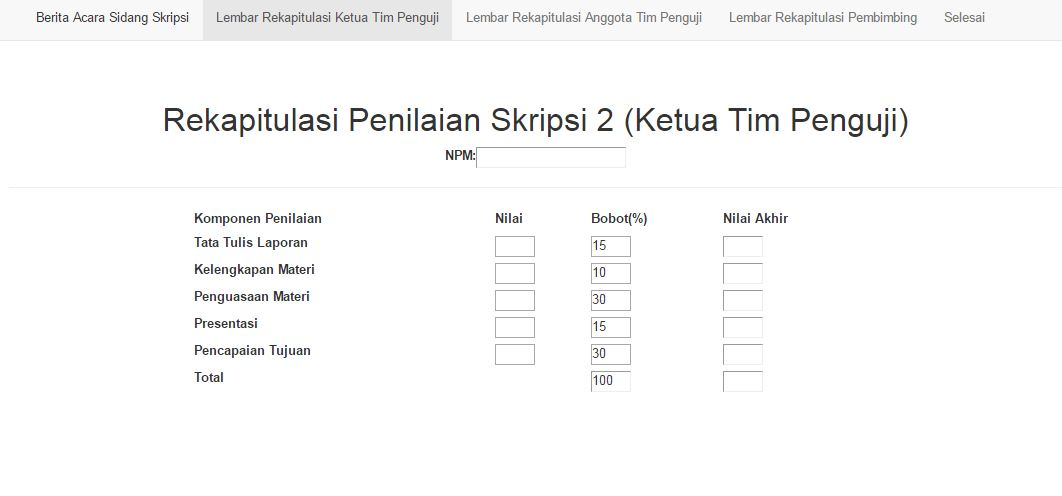
\includegraphics[scale=0.5]{Gambar/tampilanapp2}
				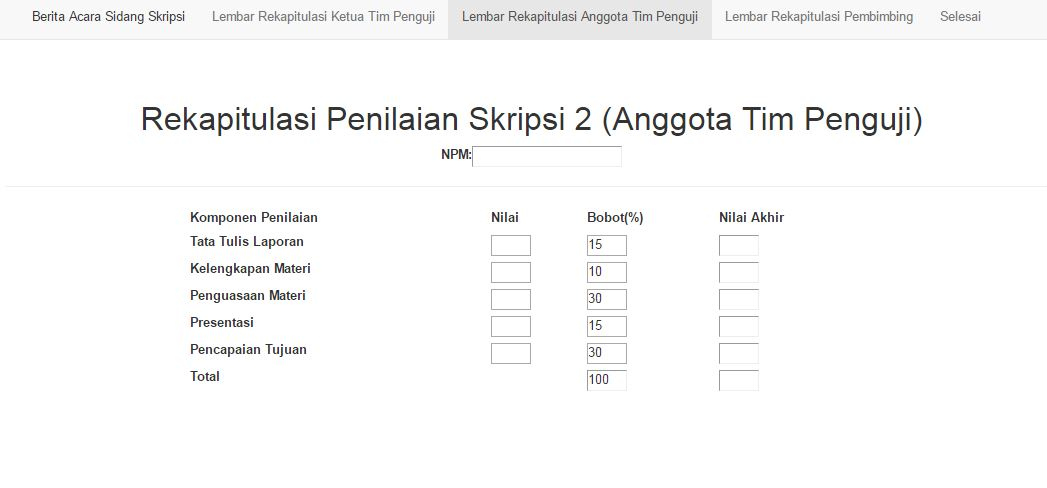
\includegraphics[scale=0.5]{Gambar/tampilanapp3}
				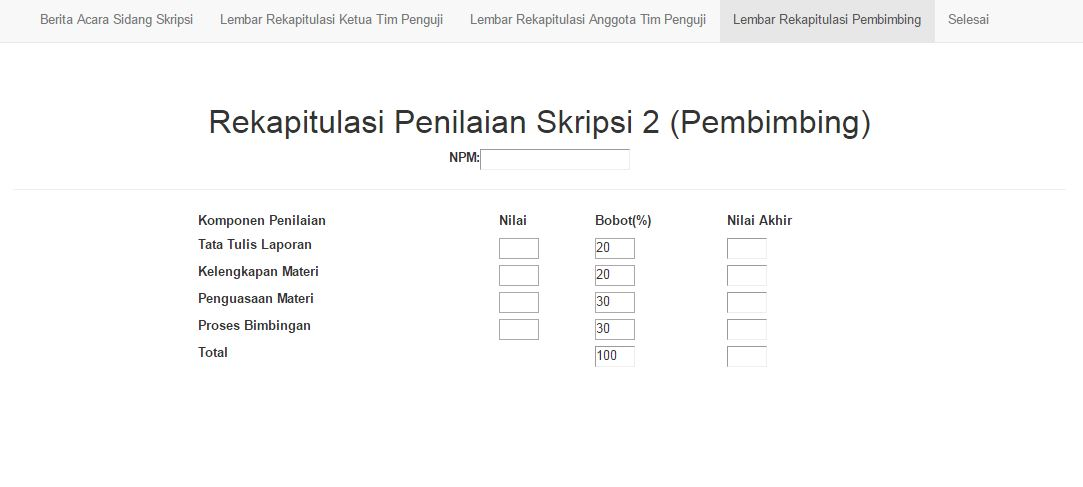
\includegraphics[scale=0.5]{Gambar/tampilanapp4}
				\caption{Gambar Tampilan Aplikasi}
				\label{fig:tampilanapp}
			\end{figure}

		\item Mengimplementasikan fitur - fitur yang ada pada form tersebut\\
		{\bf status :} Ada sejak rencana kerja skripsi.\\
		{\bf hasil :} Fitur - fitur yang terdapat pada sistem penilaian sidang skripsi 2 ini kebanyakan adalah fitur - fitur yang mengisi secara otomatis nilai - nilai pada sistem manual yang diisi oleh pengguna, contohnya adalah pengisian tanggal, pengisian NPM pada form rekapitulasi, perhitungan nilai dan total nilai, pengisian nilai default bobot per nilai, dll. Dari berbagai macam fitur yang ada pada sistem penilaian sidang skripsi 2, semua sudah dapat berjalan dengan baik sampai saat ini.  Akses ke aplikasi dapat dilakukan dengan URL "sipskripsi.com".

		\item Melakukan pengujian (dan eksperimen) pada sidang skripsi 2 semester genap 2015/2016 yang melibatkan responden untuk menilai hasil simulasi secara kualitatif\\
		{\bf status :} Ada sejak rencana kerja skripsi.\\
		{\bf hasil :} Untuk pengujian sistem penilaian sidang skripsi 2, akan diujikan pada 5 kasus sidang mata kuliah  skripsi 2 yang akan datang.

		\item Menulis dokumen skripsi\\
		{\bf status :} Ada sejak rencana kerja skripsi.\\
		{\bf hasil :} Penulisan dokumen sedang dalam perkembangan hingga bab 3.
	
	\end{enumerate}

\section{Pencapaian Rencana Kerja}
Persentase penyelesaian skripsi sampai dengan dokumen ini dibuat dapat dilihat pada tabel berikut :

\begin{center}
  \begin{tabular}{ | c | c | c | c | l | c |}
    \hline
    1*  & 2*(\%) & 3*(\%) & 4*(\%) &5* &6*(\%)\\ \hline \hline
    1   & 20  & 20  &  & & 20 \\ \hline
    2   & 15 & 5  & 10  & & 15 \\ \hline
    3   & 10  & 10  &  &  & 10 \\ \hline
    4   & 15  & 15  &   &  & 15 \\ \hline
    5   & 20 &   & 20 & & 0 \\ \hline
    6   & 20 & 	5 & 15  & {\footnotesize penulisan bab 1 pada S1}  & 10 \\\hline
    Total  & 100  & 55  & 45 &  & 70\\ \hline
                          \end{tabular}
\end{center}

Keterangan (*)\\
1 : Bagian pengerjaan Skripsi (nomor disesuaikan dengan detail pengerjaan di bagian 5)\\
2 : Persentase total \\
3 : Persentase yang akan diselesaikan di Skripsi 1 \\
4 : Persentase yang akan diselesaikan di Skripsi 2 \\
5 : Penjelasan singkat apa yang dilakukan di S1 (Skripsi 1) atau S2 (skripsi 2)\\
6 : Persentase yang sidah diselesaikan sampai saat ini 

%\section{Kendala yang dihadapi}
%%TULISKAN BAGIAN INI JIKA DOKUMEN ANDA TIPE A ATAU C
%Kendala - kendala yang dihadapi selama mengerjakan skripsi :
%\begin{itemize}
%	\item Terlalu banyak melakukan prokratinasi
%	\item Terlalu banyak godaan berupa hiburan (game, film, dll)
%	\item Skripsi diambil bersamaan dengan kuliah ASD karena selama 5 semester pertama kuliah tersebut sangat dihindari dan tidak diambil, dan selama 4 semester terakhir kuliah tersebut selalu mendapat nilai E
%	\item Mengalami kesulitan pada saat sudah mulai membuat program komputer karena selama ini selalu dibantu teman
%\end{itemize}

\pagebreak

\vspace{1cm}
\centering Bandung, \tanggal\\
\vspace{2cm} \nama \\ 
\vspace{1cm}

Menyetujui, \\
\ifdefstring{\jumpemb}{2}{
\vspace{1.5cm}
\begin{centering} Menyetujui,\\ \end{centering} \vspace{0.75cm}
\begin{minipage}[b]{0.45\linewidth}
% \centering Bandung, \makebox[0.5cm]{\hrulefill}/\makebox[0.5cm]{\hrulefill}/2013 \\
\vspace{2cm} Nama: \pembA \\ Pembimbing Utama
\end{minipage} \hspace{0.5cm}
\begin{minipage}[b]{0.45\linewidth}
% \centering Bandung, \makebox[0.5cm]{\hrulefill}/\makebox[0.5cm]{\hrulefill}/2013\\
\vspace{2cm} Nama: \pemB \\ Pembimbing Pendamping
\end{minipage}
\vspace{0.5cm}
}{
% \centering Bandung, \makebox[0.5cm]{\hrulefill}/\makebox[0.5cm]{\hrulefill}/2013\\
\vspace{2cm} Nama: \pembA \\ Pembimbing Tunggal
}

\end{document}

